\chapter{Related Work}\label{ch3}

In this chapter, the background of the emerging Internet of Things (IoT) and Fog Computing is introduced in section \ref{background}, popular IoT protocols are discussed and compared with an emphasis on The Constrained Application Protocol (CoAP) in section \ref{IoT_protocols} and \ref{CoAP_intro}, and at the end some existing implementations of CoAP are listed and discussed in section \ref{CoAP_imp}.

\section{Internet of Things (IoT) and Fog Computing} \label{background}

The Internet of Things (IoT) is a novel paradigm that is rapidly gaining ground in the scenario of modern wireless telecommunications. The basic idea of this concept is the pervasive presence around us of a variety of things or objects -- such as Radio-Frequency IDentification (RFID) tags, sensors, actuators, mobile phones, etc. -- which, through unique addressing schemes, are able to interact with each other and cooperate with their neighbors to reach common goals, without human involvement \cite{Atzori20102787}. The current revolution in Internet, mobile and machine-to-machine (M2M) technologies can be seen as the first phase of the IoT \cite{7123563}.  A growing number of physical objects are being connected to the Internet at an unprecedented rate realizing the idea of IoT. A basic example of such objects includes thermostats and HVAC (Heating, Ventilation, and Air Conditioning) monitoring and control systems that enable smart homes. Survey \cite{Atzori20102787} gives a thorough analysis on the potential application areas in IoT, including but not limited to, transportation and logistics, healthcare, smart environment (home, office, plant), industrial automation and emergency response to natural and man-made disasters where human decision making is difficult. The US National Intelligence Council (NIC) foresees that ``by 2025 Internet nodes may reside in everyday things -- food packages, furniture, paper documents, and more'' \cite{Atzori20102787}. The IoT provides a great market opportunity for equipment manufacturers, Internet service providers as well as application developers. The IoT smart objects are expected to reach 212 billion entities deployed globally by the end of 2020 \cite{gantz2012digital}. By 2022, M2M traffic flows are expected to constitute up to 45\% of the whole Internet traffic \cite{7123563}. Economic growth of IoT-based services is also considerable for businesses. Healthcare and manufacturing applications are projected to form the biggest economic impact. The whole annual economic impact caused by the IoT is estimated to be in range of \$2.7 trillion to \$6.2 trillion by 2025 \cite{7123563}.

Over the past decade, an important trend is moving computing, control, and data storage into the cloud. However, the emerging IoT introduces many new challenges that can not be adequately addressed by today`s Cloud Computing models alone. These challenges \cite{7498684} include but not limited to, stringent latency requirements under certain environment (such as industrial control systems), network bandwidth limitation due to rapid growing number of connected things, difficulty for resource-constrained devices to interact with the cloud using complex protocols, applications which require uninterrupted services but with intermittent connectivity to the cloud, and security concerns caused by the combinations of one or more issues mentioned above.

\begin{figure}[!htbp]
\centering
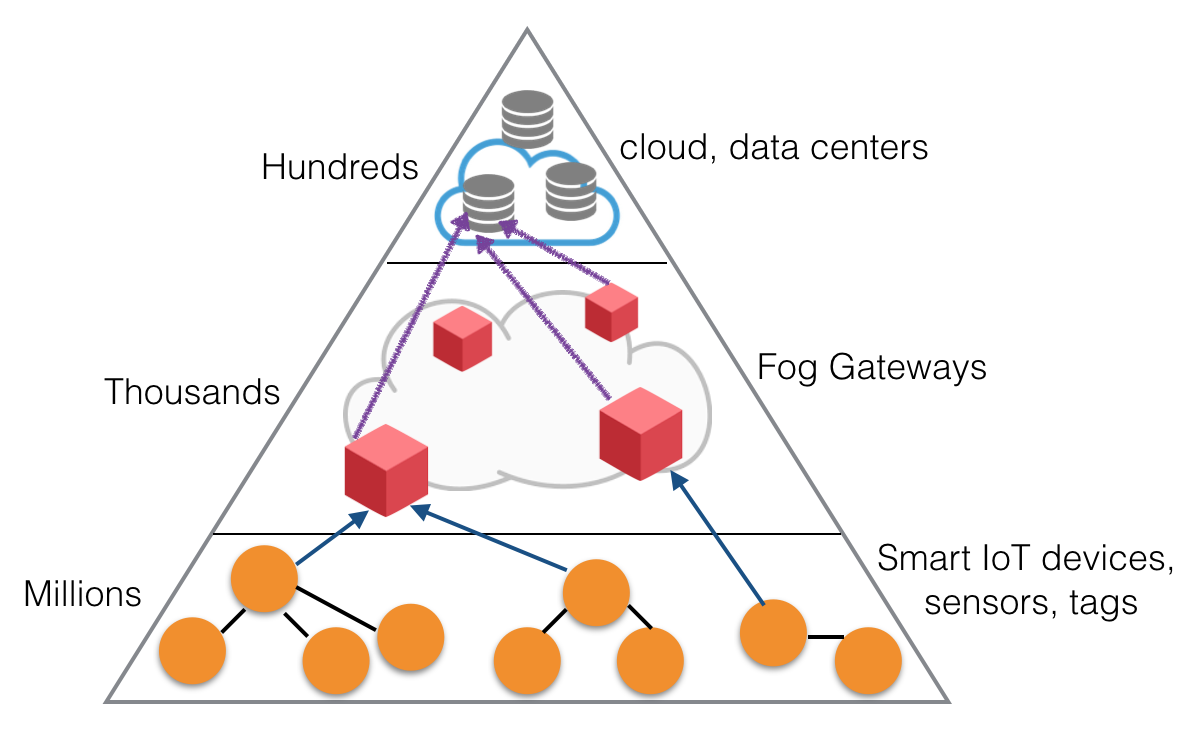
\includegraphics[scale = 0.55]{fog_computing.png}
\caption[The role of the Cloud and Fog play in the delivery of IoT services]{The role of the Cloud and Fog play in the delivery of IoT services. \cite{7123563}} 
\label{fig:fog_computing}
\end{figure}

In order to filling the technology gaps in supporting the IoT, a new architecture - Fog - was first introduced. In contrast to traditional cloud model, where many sensors upload raw data directly to a central cloud infrastructure for further processing and analysis, Fog is a highly virtualized platform that provides compute, storage, and networking services between end devices and traditional Cloud Computing data centres, which, typically but not exclusively located at the edge of network \cite{Bonomi:2012:FCR:2342509.2342513}.  Fog consists of heterogeneous, potentially wide-spread and geographically distributed networks of nodes, where a node can be any smart edge device or system that acts as a local control centre for all related sensors and actuators. A Fog in each location can be as small as a single node or as large as required to meet customer demands and a large number of small Fog nodes may form a large Fog system \cite{7498684}. 

Due to the characteristics of Fog, it enables IoT applications which require low-latency, location-awareness, real-time interactions and analytics and mobility support. Fog also enhances scalability and resilience of IoT applications by its nature \cite{7123563}. Various services and computing tasks can run on a fog node, depending on how much resource a node owns and application requirements. Applications could on one hand let local Fog carry out resource-intensive tasks (M2M interaction, data collection and processing, actuator control, etc.) on behalf of resource-constrained devices when such tasks can not be moved to cloud due to latency constraints or any other reason, on the other hand expect the preprocessed data to be consumed by higher tiers, which can be other Fog or the global Cloud, for long-term analysis and storage \cite{Bonomi:2012:FCR:2342509.2342513}\cite{7498684}. Figure \ref{fig:fog_computing} illustrates the roles that the Cloud data centres and the Fog play to deliver IoT services to end-users. 

Fog Computing has the potential to increase the overall performance of IoT applications as it tries to perform part of high level services which are offered by cloud inside the local resources \cite{7123563}. Typical Fog applications include Connected Vehicle (CV), Smart Grid and wireless sensors (actuators) networks \cite{Bonomi:2012:FCR:2342509.2342513}. A real world success of Fog has been discussed in \cite{7498684}, where Barcelona utilized Fog as a uniform platform for all services in their smart city management applications and reduced overall system costs.

Fog Computing provides a new application scenario for this work. Scalability and reliability is still required on a Fog node especially when complex tasks and services being deployed. The Fog node is highly possible a less-constrained embedded device such as the Raspberry Pi \cite{raspberry_pi}, which has more resources than common sensors and actuators yet is much less powerful than the Cloud. Moreover,  since CoAP is a standard M2M protocol, it surely has its use space under a Fog environment. Thus the combination is not only a valid use case in terms of Fog Computing, but also falls into the scope of this thesis. A detailed evaluation of the proposed CoAP server on Raspberry Pi is stated in chapter \ref{ch5}.

\section{Application Protocols for IoT} \label{IoT_protocols}

The IoT will be made up of large number of heterogeneous devices, which are equipped with extremely diverse capabilities, in terms of processing power, connectivity, availability, and mobility. In order to effectively allow and foster the growth of new applications and services, it is necessary to provide appropriate standards that can guarantee full interoperability among existing hosts and IoT nodes \cite{cirani2015mjcoap}. 

Many standards around the IoT have been introduced to facilitate and simplify application programmers' and service providers' jobs. While many efforts have been made to bring Internet Protocol (IP) to all kinds of devices so that they can be part of the existing Internet, application layer protocols are another important part of these standards.

In general, current IoT application protocols can be divided into 3 types: message-oriented, data-oriented, and resource-oriented \cite{7396558}. Representative protocols of the 3 types are Message Queue Telemetry Transport (MQTT) \cite{mqtt_protocol}, Data Distribution Service for Real Time Systems (DDS) \cite{dds} and The Constrained Application Protocol (CoAP) \cite{coap_protocol}. In this section, these protocols are discussed and compared in terms of their architecture and use cases. 
Reason for choosing CoAP as the protocol used in this work is also stated. 

\subsection{Message-oriented:  Message Queue Telemetry Transport (MQTT)}
Publish/subscribe messaging is one of the most common message-oriented architectures, where subscribers specify their interest in messages of certain type or topic, and receive messages asynchronously once a publisher publishes a message on the registered interest \cite{6918928}. Usually the only property a publisher needs in order to communicate with a subscriber is the name and definition of the data. The publisher does not need any information about the subscribers, and vice versa \cite{pardo2005introduction}. Under message-oriented paradigm, MQTT is outstanding for its simplicity and efficiency, which costs only a small footprint and low power consumption on embedded devices, meanwhile guarantees the reliability and flexibility for message distribution.

MQTT is a messaging protocol that was introduced by Andy Stanford-Clark of IBM and Arlen Nipper of Arcom (now Eurotech) in 1999 and was standardized in 2013 at OASIS \cite{mqtt_protocol}. It aims at connecting embedded devices and networks with applications and middleware. The connection operation uses a routing mechanism (one-to-one, one-to-many, many-to-many) and enables MQTT as an optimal connection protocol for the IoT and M2M \cite{7123563}. 

\begin{figure}[!htbp]
\centering
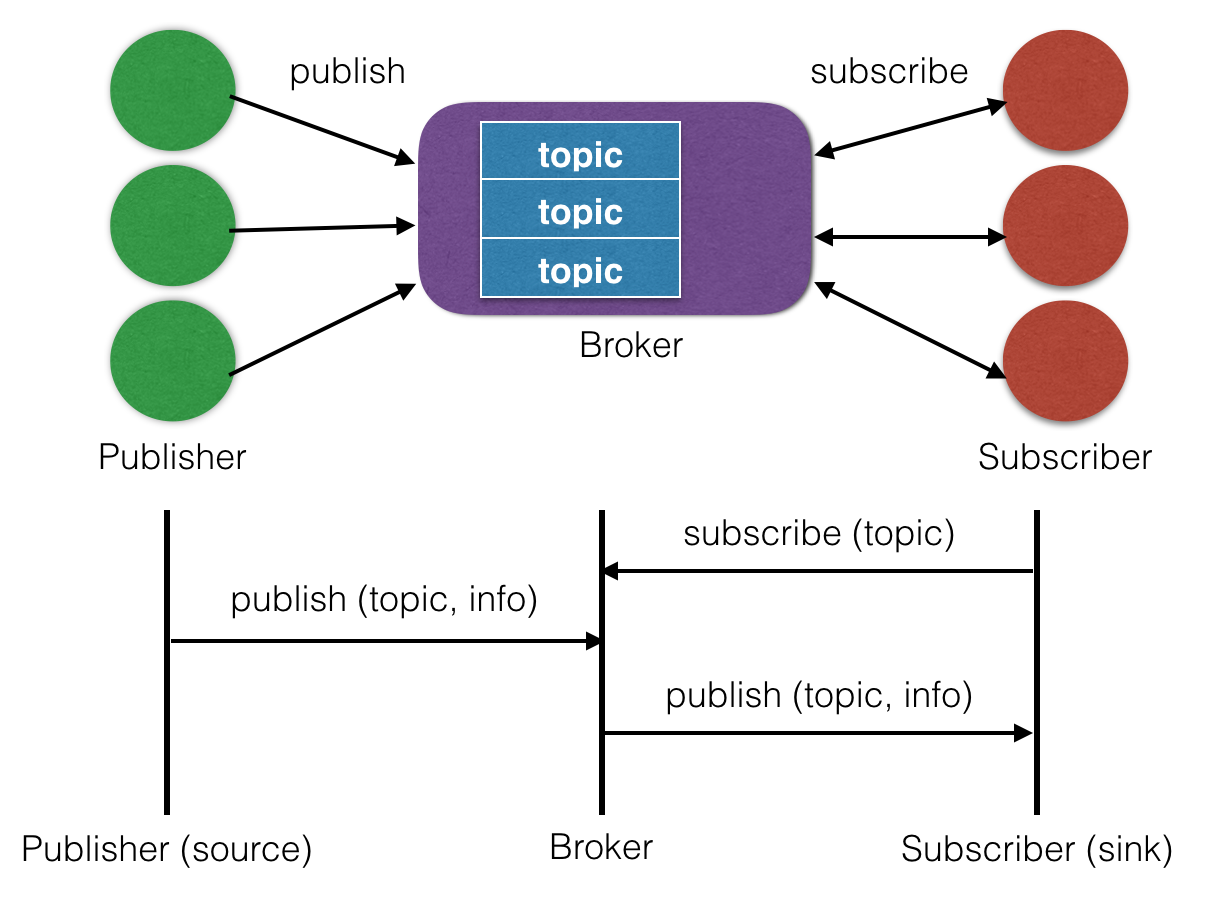
\includegraphics[scale = 0.55]{mqtt.png}
\caption{The architecture of MQTT and its publish/subscribe process}
\label{fig:mqtt}
\end{figure}

MQTT is based on topic based publish-subscribe architecture with a message-broker to bridge between the publishers and subscribers, as shown in figure \ref{fig:mqtt}. It exploits the decoupling in space, time and flow as the core of its working philosophy. An interested device would register as a subscriber for specific topics in order for it to be informed by the broker when publishers publish topics of interest. The publisher acts as a generator of interesting data. After that, the publisher transmits the information to the interested entities (subscribers) through the broker. Furthermore, the broker achieves security by checking authorization of the publishers and the subscribers \cite{4554519}\cite{6504105}.

MQTT supports 3 QoS (Quality of Service) levels for message delivery with enhanced reliability and has a low header overhead \cite{mqtt_protocol}. MQTT is a connection oriented protocol as the publisher or the subscriber both needs persistent connection to the message broker. It relies on the underlying TCP layer for connection features \cite{6504105}. This in turn can lead to challenges with respect to communication costs. Consequently a UDP based MQTT for sensors (MQTT-S) \cite{4554519} was developed.

\subsection{Data-oriented: Data Distribution Service (DDS)}

Tijero \cite{tijero2012schedulability} and Pardo-Castellote \cite{pardo2005introduction} pointed out that Data Distribution Service for Real Time Systems (DDS) applies a data-oriented/data-centric paradigm. Data-centric communication provides the ability to specify various parameters like the rate of publication, rate of subscription, how long the data is valid, and many others. These Quality of Service (QoS) parameters allow system designers to construct a distributed application based on the requirements for, and availability of, each specific piece of data.

DDS is a publish-subscribe protocol for real-time M2M communications that has been developed by Object Management Group (OMG) \cite{dds}. In contrast to other publish-subscribe application protocols like MQTT, DDS relies on a broker-less architecture and uses multicasting to bring excellent Quality of Service (QoS) and high reliability to its applications \cite{7123563}. Its broker-less architecture fits well with the real-time requirements for IoT and M2M communications. DDS supports 23 QoS policies by which a variety of communication criteria like security, urgency, priority, durability, reliability, etc. can be addressed by the developer \cite{7123563}. In short, DDS has the following advantages \cite{pardo2005introduction}:

\begin{itemize}
\item Based on a simple ``publish-subscribe'' communication paradigm
\item Flexible and adaptable architecture that supports ``auto-discovery'' of new or stale endpoint applications
\item Low overhead -- can be used with high-performance systems
\item Deterministic data delivery
\item Dynamically scalable
\item Efficient use of transport bandwidth
\item Supports one-to-one, one-to-many, many-to-one, and many-to-many communications
\item Large number of configuration parameters that give developers complete control of each message in the system
\end{itemize}

It is important to note that OMG's DDS specification is silent on the wire-protocol. This in turn has led to the problem that DDS products from different vendors face interoperability issues. To overcome these interoperability issues OMG promotes the use of Real-Time Publish-Subscribe protocol (RTPS) \cite{rtps} as a wire-protocol for DDS. RTPS itself relies on the use of UDP and multicast to deliver the data from publishers to subscribers. Depending on the network-topology and routers used, RTPS can deliver impressive throughput. 

An experimental evaluation of two implementations of DDS \cite{4536566} points out that this protocol scales well when the number of nodes is increased. While DDS inspired/compatible protocols have been proposed for wireless and sensor scenarios, there seems to be a lack of successful deployments \cite{7396558}, partly due to its complexity. 

\subsection{Resource-oriented: the Constrained Application Protocol (CoAP)}

IoT applications usually consist of myriads of devices that have minimal unit costs, which means they are constrained in power supply, available memory footprint, processing capabilities and much more. These constrained devices can surely benefit from a connection to the Internet as they can be integrated into distributed services. The Internet Engineering Task Force (IETF) has already undertaken much standardization work to make it happen. The IPv6 over Low-Power Wireless Area Networks (6LoWPAN) standards (RFCs 4944 and 6282) now enable IPv6 even on very constrained networks, which allows for seamless integration of sensor and actuator nodes into the Internet \cite{6159216}. 

For full convergence, however, devices and services must also interoperate at the application layer \cite{kovatsch2014californium}. When it comes to mashing up of different services, the World Wide Web has proven its scalability and flexibility. Many applications today depend on the Web architecture, using HTTP to access information and perform updates. HTTP over TCP has problems in constrained environment, though, not only because its overhead in implementation code space, but also low network resource usage due to the fact that high packet error rates and lossy links are common in constrained networks \cite{6159216}. To come over such a gap, the IETF designed a new Web protocol from scratch, the Constrained Application Protocol (CoAP). 

CoAP follows the Representational State Transfer (REST) \cite{fielding2000architectural} like HTTP, but is tailored to the requirements of constrained devices and networks. A compact binary format is employed and the protocol runs over UDP (or Datagram Transport Layer Security (DTLS) when security is enabled). A messaging sub-layer provides duplicate detection and optional reliable delivery of messages, based on a simple stop-and-wait mechanism for retransmissions. On top of it, the request/response sub-layer enables RESTful interaction with the web in a similar fashion as HTTP \cite{kovatsch2014californium}. That being said, CoAP is primarily based on patterns from the Web: a client/server interaction model between application endpoints, resources that are addressable by Uniform Resource Identifiers (URIs), stateless exchange of representations that decouple client and server, uniform interfaces with standardized Internet Media Types for wide interoperability, and caching and proxying to enable high scalability \cite{kovatsch2015scalable}. 

CoAP is not a mere compression of HTTP, but goes beyond that. For instance, it supports group communication through the underlying UDP; resources are \textit{observable} \cite{coap_observe}, that is, extra responses continuously push state changes to all registered clients; it includes a machine-to-machine discovery mechanism to find matching resources based on Web Linking \cite{core}; application-layer fragmentation allows blockwise on-the-fly processing of messages that would otherwise exceed the maximum transmission unit (MTU) \cite{blockwise}; alternative transports such as Short Message Service (SMS) or Unstructured Supplementary Service Data (USSD) are also possible and are under standardization \cite{coap_alter_trans}.

Since both CoAP and HTTP all follow the REST style, CoAP can easily be mapped to HTTP and be connected via transparent proxies and integrated into the same system. A typical CoAP application architecture is shown in figure \ref{fig:coap_app_architecture}. The core of the protocol is specified in RFC 7252 \cite{coap_protocol}, important extensions are in various stages of the standardization process. 

\begin{figure}[!htbp]
\centering
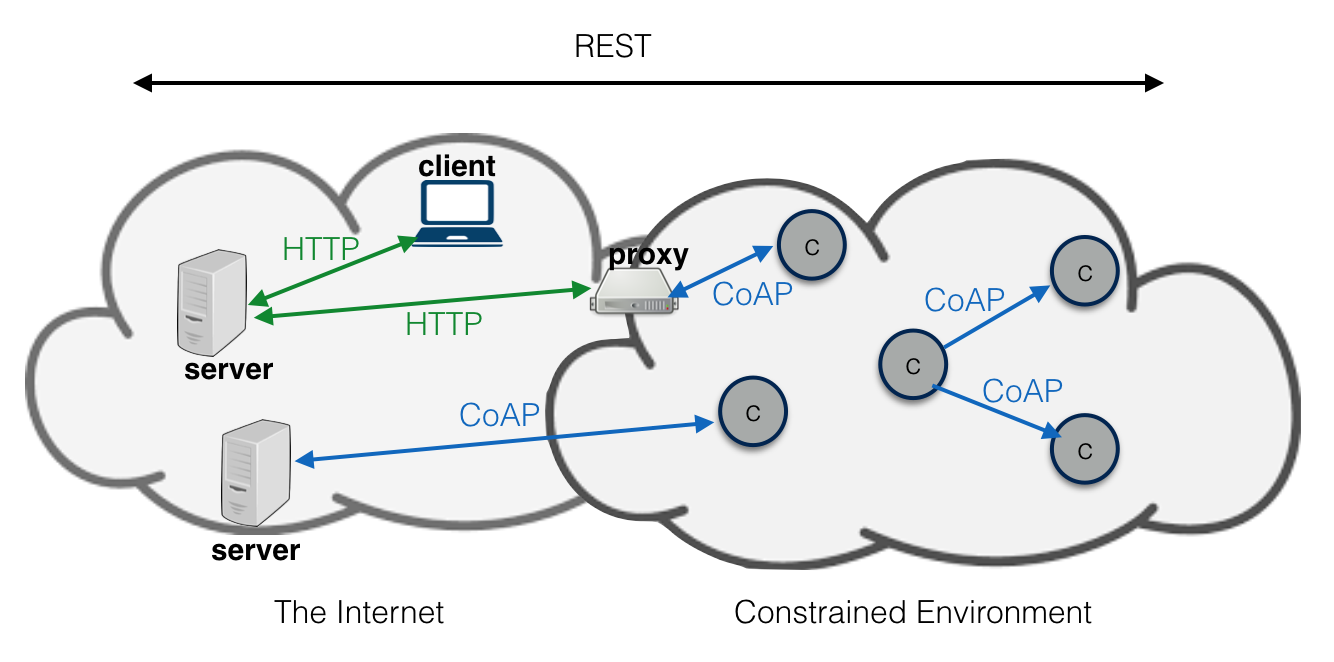
\includegraphics[scale = 0.55]{coap_app_architecture.png}
\caption{A typical CoAP application architecture}
\label{fig:coap_app_architecture}
\end{figure}

\subsection{Comparison}
%In this section, a brief comparison of MQTT, DDS and CoAP is given. 

Speaking of CoAP and MQTT, CoAP seems to have a wider acceptance for constrained devices due to the following facts: ease of integration with 6LowPAN, easy portability with HTTP, UDP based operation with low connection overhead, support for several features like sleeping nodes \cite{coap_protocol}(without requiring persistent connection), support for both request-response and resource-observe mode. On the other hand, MQTT is ideal for integration with existing cloud service since TCP is already employed in most infrastructures. 

MQTT is a message-oriented protocol which means that it is content agnostic and only focusses on the delivery of messages, while CoAP is all about operations against the representation of resource since it follows the REST style. Resource observing in CoAP is similar to publish/subscribe feature in MQTT at first glance, but unlike publish/subscribe, where the goal is to propagate every event, observe only guarantees that eventually all registered observers will have a current representation of the latest resource state. As a result of forementioned difference, MQTT is simple to implement on the sensor/device side since all relevant part is about message delivery. Reference \cite{6918928} pointed out several disadvantages of resource-oriented IoT protocol like CoAP, including overhead introduced to constrained devices in terms of concurrency, computing and networking, inflexibility that IP address of each device must be known, as well as Network Address Translation (NAT) issue for global accessibility in currently most common IPv4 subnet environment. 

However, CoAP has a clear semantics of operations against a resource and different CoAP method can be used to differ read and write. While MQTT's publish/subscribe architecture results in a non-intuitive way of communication when the subscriber also needs to send feedback of configuration command to the publisher, since it is not the default message flow direction. Moreover, MQTT differs a lot in terms of finding services. With MQTT, it is necessary to first find the central server, a.k.a., the broker and messages always go through the broker. There is no need for a central endpoint for CoAP since it supports multicast to discover available services. And after that, the read/write semantics of CoAP ensures independent communication endpoint to endpoint. That is to say, it requires less effort to make CoAP scale up than MQTT. Matthias Kovatsch \cite{kovatsch2015scalable} stated similar argument that the main drawback of MQTT is missing extensibility, as MQTT clients must be pre-configured with a dedicated service like HTTP clients for IoT, which makes it hard to adapt to an evolving environment.

There are few research publications as well as industry deployments about DDS, which implies it may be still under exploration and optimization stage. On the other hand, there are known scalability \cite{esposito2011data} and performance \cite{sanchez2011bloom} issues associated with RTPS, which is the wire-protocol used in DDS. Also, DDS's Global Data Space (GDS) concept is of limited use when faced with unreliable, low bandwidth and high latency networks \cite{7396558}.

\begin{table}[!htbp]
\newcolumntype{Y}{>{\centering\arraybackslash}X}
\begin{tabularx}{\textwidth}{l|c|c|c|c|c|c|c|Y}
%
			& Transport 			& RESTful 	& \makecell{Publish/\\Subscribe} 	& \makecell{Request/\\Response} 	& \makecell{Central\\Broker} 	& \makecell{Header\\Size\\(bytes)} 	& Security & Reliability \\ \hline
MQTT 		& TCP 				& \XSolid 		& \Checkmark 					& \XSolid 						& \Checkmark 				& 2 & SSL & 3 QoS levels \\ \hline
DDS 		& \makecell{TCP\\UDP} 	& \XSolid 		& \Checkmark 					& \XSolid 						& \XSolid 					& - & \makecell{SSL\\DTLS} & 23 QoS policies \\ \hline
CoAP 		& UDP 				& \Checkmark 	& \Checkmark					& \Checkmark 					& \XSolid 					& 4 & DTLS & Simple stop-and-wait retransmission reliability with exponential back-off  \\  \hline
HTTP 		& TCP 				& \Checkmark 	& \XSolid 						& \Checkmark 					& - 						&  - 	& SSL & - \\ 
\end{tabularx}
\caption{A brief comparison between MQTT, DDS and CoAP}
\label{tab:mqtt_dds_coap}
\end{table}

\begin{table}[!htbp]
\centering
\begin{tabular}{l|p{5.8in}}
%\hline
%
& \multicolumn{1}{c}{Typical application} \\ \hline
MQTT & Topic based real-time messaging kind of application using pub/sub requiring persistent connection with the server. Message broker is responsible to weave the sensors with the rest of the Web. \\ \hline
DDS & Applications and system-of-systems using pub/sub that have to be able to support dynamically changing environments and configurations, be constantly available, and be instantly responsive. Integrating data across many platforms and disparate systems is also necessary. \\ \hline
CoAP & Applications with sensors running RESTful web-services to achieve direct connectivity to the Web with HTTP like methods and URI. Applications integration with HTTP based Web. \\
\end{tabular}
\caption{Potential usage of MQTT, DDS and CoAP}
\label{tab:mqtt_coap_dds_app}
\end{table}

Table \ref{tab:mqtt_dds_coap} provides a brief comparison between MQTT, DDS, CoAP and HTTP in terms of architecture. HTTP is also included here as a contrast to CoAP since they share many similarities. Table \ref{tab:mqtt_coap_dds_app} provides the potential application areas of the three protocols.

The resource-oriented pattern in general provides a more intuitive abstraction when linking devices to the Internet. The Web is a loosely-coupled application layer architecture \cite{6159216} and so is the IoT. It is easy for such a pattern to interwork with existing Web. With such a pattern, devices connected to the Internet are viewed as unique resources (identified by URIs) and accessed through well-known methods (such as GET, PUT, POST, and DELETE) with a clear semantics about read/write and representation state (controlled by Internet Media Types). 

A particularly interesting aspect of the resource-oriented communication is the natural emergence of Fog Computing. Since the resources need to process the requests, they must have some basic processing capabilities. This in turn allow us to distribute the processing load and to reduce the load on backend-services. In addition, since the requests have a clear read/write semantic, it becomes possible to add infrastructure support in form of caching and reverse proxies thus allowing for more distribution of load and network traffic \cite{7396558}. 

There is no IoT application protocol that fits all situations. As A. Al-Fuqaha et al. \cite{7123563} pointed out, gateways that could interoperate with many different IoT protocols are under active research so that protocols can be deployed with much more flexibility. Speaking of CoAP, it makes it easy for applications that are more likely deployed in unconstrained environment to talk to constrained devices. It also provides observe functionality when publish/subscribe pattern is more a desired goal. More importantly, CoAP has its position in both Fog and Cloud and consequently has been selected as the protocol used in this thesis.


\section{CoAP Fundamentals and Implementations} \label{CoAP_intro}

This section gives an inspection of some key features and concerns of CoAP, which will define the important terminology for this research and give insight of ideas and trade-off made in the proposed architecture that is discussed with more details in later chapters. It is followed by a brief analysis of available implementations which also shows the position of this work. 

In detail, target environment of CoAP is defined in \ref{CORE_env}; basic semantics of the core protocol is introduced in \ref{core_protocol}; an important extension of the core protocol - observe is discussed in \ref{observe_resource}; security issue is covered in \ref{security}; a more detailed comparison with HTTP is stated in \ref{vs_HTTP} which also acts as a brief summary of above sections; and a summary of current implementations is in \ref{CoAP_imp}.

\subsection{Constrained RESTful Environments}\label{CORE_env}

In order to provide a framework for applications that embrace constrained IP networks as found in the IoT,  the working group for Constrained RESTful Environments (CoRE) considers it is necessary to classify resource-constrained devices according to their capabilities. RFC 7228 on terminology defines the following 3 classes \cite{constarined_env}\cite{kovatsch2015scalable}:

\begin{itemize}

\item \textbf{Class 0} devices are very constrained sensor-like motes.  They are so severely constrained in memory and processing capabilities that most likely they will not have the resources required to communicate directly with the Internet in a secure manner.  To participate in Internet communications, Class 0 devices require the help of larger devices acting as proxies, gateways, or servers. Obvious examples are proprietary temperature sensors that send their readings wirelessly to an indoor weather station or bedside alarm clock. Their memory sizes are usually in the order of hundreds of bytes only.

\item \textbf{Class 1} devices are most resource-constrained devices that can directly connect to the Internet with on-board security mechanisms, which requires about 100 KB of ROM and about 10KB of RAM.  They can not employ a full protocol stack such as using HTTP, Transport Layer Security (TLS), and related security protocols and XML-based data representations, due to limited memory size and processing power. Hence they require lightweight protocols that have low memory footprints and parsing complexity, such as CoAP.

\item \textbf{Class 2} devices are less constrained and almost show the characteristics of full-fledged Internet nodes like smartphones or notebooks. This becomes possible at about 250 KB of ROM and about 50 KB of RAM. Yet, even these devices can benefit from lightweight and energy-efficient protocols and from consuming less bandwidth, in order to free resources for the application or reduce operational costs. Constrained devices with capabilities more than Class 2 exist but they can still be constrained by a limited energy supply.

\end{itemize}

According to above definitions, sensors and actuators are more likely to be class 0 devices. And some System on Chip (SoC) falls into class 1 and may operate on behalf of the class 0 devices and expose their resources to outside world. Other embedded platform such as mobile phones and the Raspberry Pi \cite{raspberry_pi} can be seen as class 2 or beyond. They could thus perform more complex tasks and make real-time decisions based on information provided by potentially many class 0 and class 1 devices. Such a hierachical structure also naturally fits into the definition of a Fog. In the thesis, the Raspberry Pi is used as the evaluation platform for constrained environment since it is more likely to deal with lots of concurrent clients/servers and has the potential to do some simple preprocessing other than just protocol handling.


\subsection{Core Protocol}\label{core_protocol}

CoAP is designed to use minimal resources, both on the device and on the network. Instead of a complex transport stack, it gets by with UDP on IP. A 4-byte fixed header and a compact encoding of options enables small messages that cause no or little fragmentation on the link layer. Figure \ref{fig:msg_format} \cite{coap_protocol} shows the four-byte base header of CoAP, which can be followed by the variable-length token, multiple header options, and a payload carrying the representations mentioned above.

\begin{figure}[!htbp]
\centering
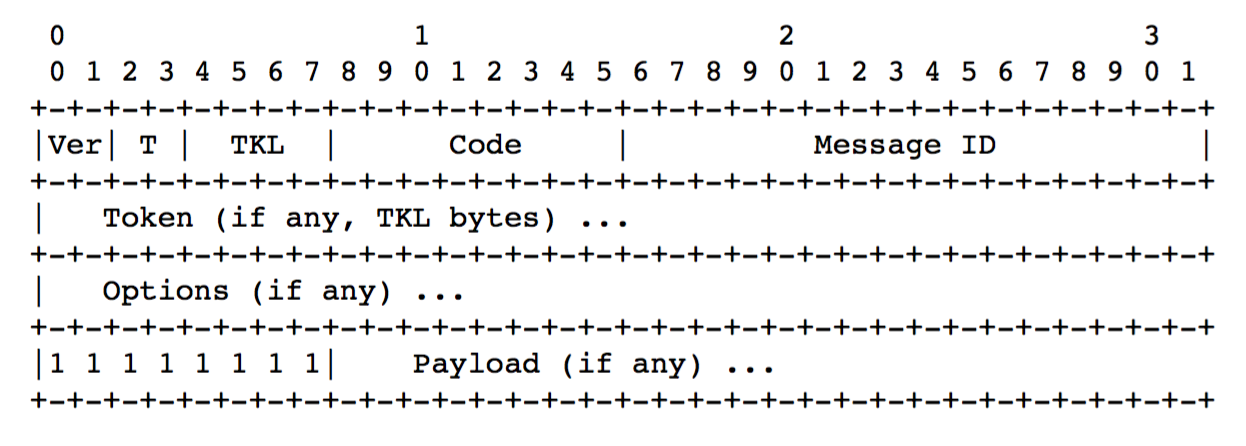
\includegraphics[scale = 0.55]{msg_format.png}
\caption{Message format}
\label{fig:msg_format}
\end{figure}

An entity participating in the CoAP protocol is called an endpoint \cite{coap_protocol}. It lives on a network node and is identified by its IP address, port, and security association. One can think CoAP of as having two sublayers: the request/response-layer and the message-layer, as shown in figure \ref{fig:coap_layer} \cite{coap_protocol}.

\begin{figure}[!htbp]
\centering
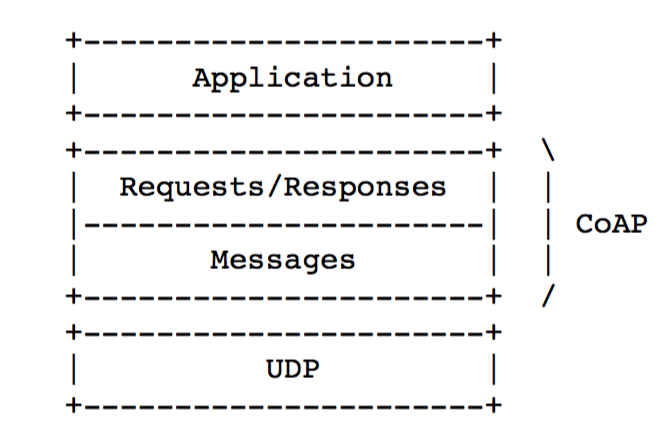
\includegraphics[scale = 0.55]{coap_layer.png}
\caption{Abstract layering of CoAP}
\label{fig:coap_layer}
\end{figure}

Messages can either be confirmable (CON), non-confirmable (NON), acknowledgements (ACK) or resets (RST). Confirmable and non-confirmable messages carry requests or responses. When an endpoint receives a confirmable message, it replies with an acknowledgement. The response to a confirmable request can be sent with the ACK, which is also called piggybacked response, or in a separate confirmable response. An endpoint retransmits confirmable messages with an exponentially increasing back-off timer until it receives an acknowledgement, a reset or the maximum retransmission count is reached (which is typically 4). If an endpoint receives a CON or NON that it does not know how to process, it rejects it with a RST. A message is identified by a message ID (MID) and an endpoint needs to temporarily remember incoming MIDs to detect duplicates. For a confirmable request, one endpoint only considers successfully receiving an acknowledgement when receiving ACK with the same MID as in the request, which is 0x7d34 in the example in figure \ref{fig:reliable_msg_trans} \cite{coap_protocol}. For a non-confirmable request, no ACK is required and MID is only used to detect duplicates, as shown in figure \ref{fig:unreliable_msg_trans} \cite{coap_protocol}.

\begin{figure}[!htbp]
\begin{subfigure}[t]{.5\textwidth}
  \centering
  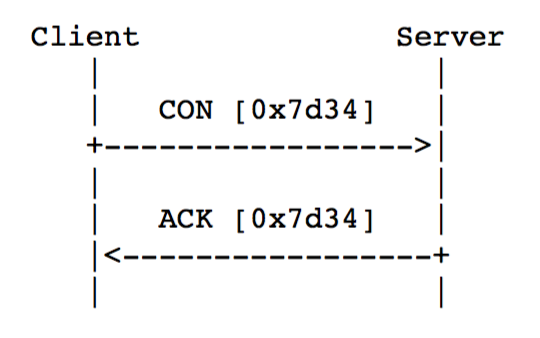
\includegraphics[scale = 0.55]{reliable_msg_trans.png}
  \caption{Reliable}
  \label{fig:reliable_msg_trans}
\end{subfigure}%
\begin{subfigure}[t]{.5\textwidth}
  \centering
  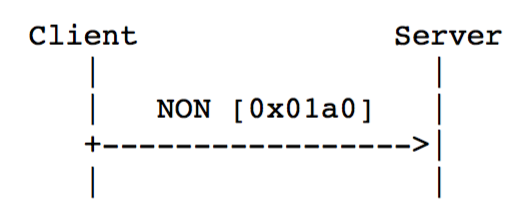
\includegraphics[scale = 0.55]{unreliable_msg_trans.png}
  \caption{Unreliable}
  \label{fig:unreliable_msg_trans}
\end{subfigure}
\caption{Reliable and unreliable message transmission}
\end{figure}

\begin{figure}[!htbp]
\centering
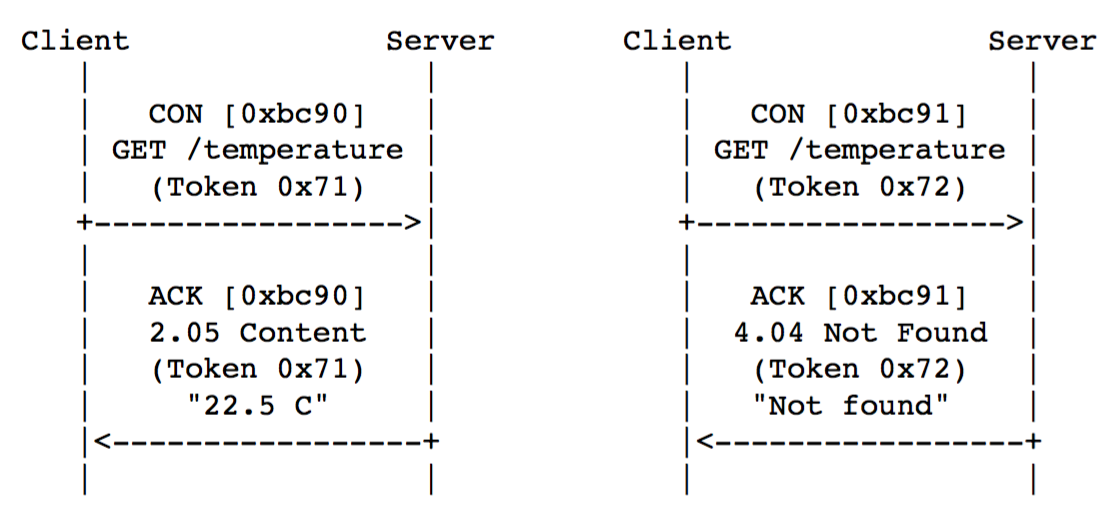
\includegraphics[scale = 0.55]{get_example.png}
\caption{Two GET requests with piggybacked responses}
\label{fig:get_example}
\end{figure}

On the request/response-layer, requests have a method code (GET, POST, PUT, or DELETE) and responses have a response code (either of class 2.xx (success), 4.xx (client error), or 5.xx (server error)). A token, chosen by the client, serves as identifier for a request. The server endpoint must include the request token in the response so that the client endpoint knows to which request the response belongs to. Additionally, CoAP requests and responses can be accompanied by simple options, similar to HTTP header options. For example, options may describe the content format or destination URI. Two examples for a basic GET request with piggybacked response are shown in Figure \ref{fig:get_example} \cite{coap_protocol}, one successful, one resulting in a 4.04 (Not Found) response.

\subsection{Observing Resources}\label{observe_resource}

A key feature for the IoT is observing resources. The observe extension enables efficient server push notifications based on the observer pattern \cite{kovatsch2015scalable}. It is designed as an optional feature on top of GET with an elective Observe option that is set to zero by the client. If a server does not support it, this is as answering a normal GET request and clients can repeat requesting to polling. When the server supports this feature, it will respond with this option, which turns the response into a notification. The server promises to keep the interested client on its list of observers as long as possible and will push new representations whenever the observed resource changes. This extends the request-response pattern to a request/multiple-response pattern, where all notifications are correlated as usual through the token. CoAP notifications also make use of cache control, that is, they have a valid lifetime defined by the Max-Age option and are cacheable. Usually the server sends a new representation before Max-Age expires. When a representation becomes stale, the client assumes that it was dropped by the server (e.g., because of a reboot) and can re-register by sending another observe request using the same token. Also the options must be identical to the original observe registration, so that the request matches the cache key in case intermediaries are involved.

\begin{figure}[!htbp]
\centering
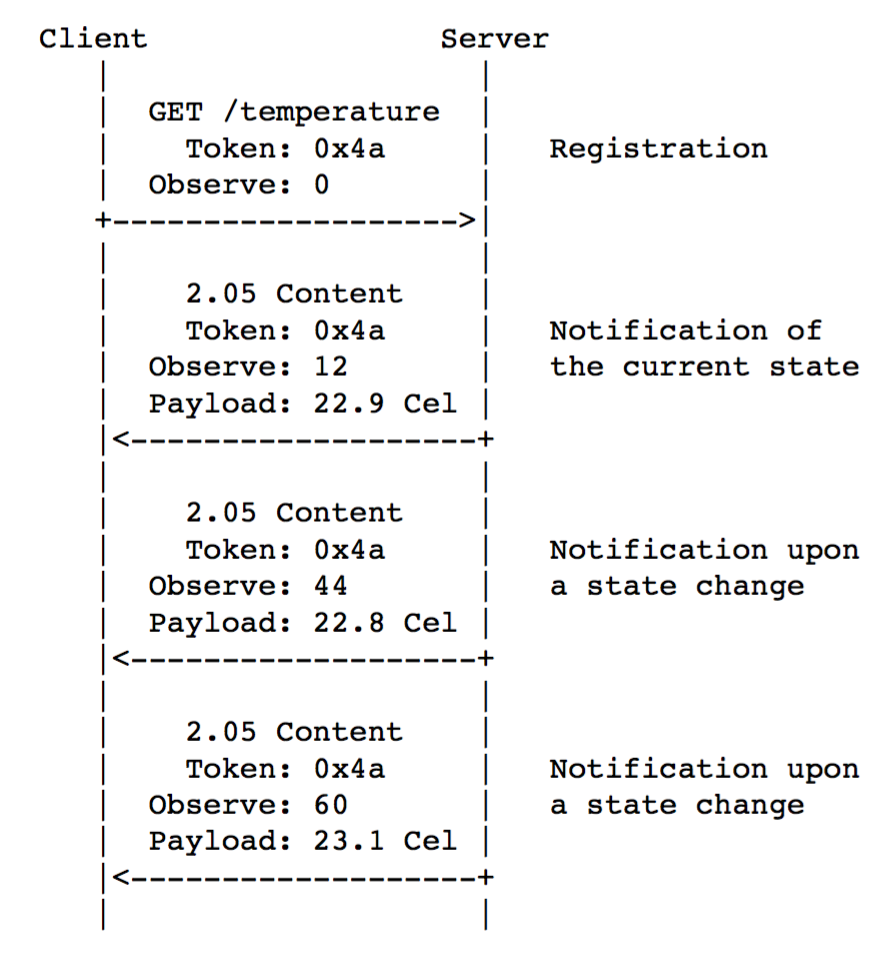
\includegraphics[scale = 0.55]{coap_observe.png}
\caption[CoAP observe synchronization]{CoAP observe synchronizes the local state with the resource state at the origin server by sending push notifications. \cite{coap_observe}}
\label{fig:coap_observe}
\end{figure}

In case the client is no longer interested, there are two possibilities to end an observe relationship \cite{kovatsch2015scalable}:

\begin{itemize}

\item \textbf{Re-active cancellation:} Observers can simply remove the local relationship states, which leads to a ``garbage collection" at the server: When the next notification arrives, the client cannot match the token and will reject it. Since every once in a while the server must use a CON notification to detect orphans, it will eventually receive a RST that tells the server to remove the client from its list of observers. The same happens when a CON transmission times out, usually caused by a client that shut down (orphan).

\item \textbf{Pro-active cancellation:} Some applications require a more timely cancellation to save resources. In this case, clients can send a cancellation request by setting the Observe option to one and using the token associated with the relationship.

\end{itemize}

\subsection{Security}\label{security}

The security model of CoAP is similar to traditional Web services: Transport Layer Security (TLS). Due to the resource constraints and UDP binding, CoAP depends on Datagram Transport Layer Security (DTLS) for security (see section 9 of \cite{coap_protocol}). It provides the same flexibility with a variety of cipher suites, which define the set of cryptographic algorithms used. The DTLS In Constrained Environments (DICE) Working Group of the Internet Engineering Task Force (IETF) works on supporting the use of DTLS in constrained environments.  The integration of DTLS into the Java CoAP implementation Californium \cite{californium} is discussed in a master's thesis from 2012 \cite{jucker2012securing}. Since DTLS adds extra complexity and may degrade performance of a CoAP server, various optimization should be taken into account and thus it is not a focus of this work.

\subsection{CoAP vs. HTTP}\label{vs_HTTP}

It is important to note that CoAP is more than just a compressed form of HTTP and moreover provides several features that are beneficial in an M2M application. Reference \cite{lanter2013scalability} gives a comprehensive comparison between CoAP and HTTP in terms of protocol concept as well as the processes for handling requests on server side. It shows how CoAP + UDP are superior to HTTP + TCP in constrained environments. In short, the similarities and differences are,

\begin{itemize}
\item \textbf{Fewer messages}: A typical CoAP exchange consists of 2 messages, i.e., a request and a response. In contrast, an HTTP request first requires the client to establish a TCP connection and later terminate it. CoAP's blockwise transfer\cite{blockwise} though, requires an acknowledgement for each block and leads to more messages and higher transfer time. But since most CoAP messages are short, this is not a big concern.

\item \textbf{Compressed format}: CoAP encodes option values in binary format while an HTTP request is one large, verbose text. A minimum CoAP header is only 4 bytes long and a minimum UDP header is only 8 bytes long. In contrast, a minimum TCP header alone is 20 bytes long plus what comes from HTTP. A bare CoAP request is not human-readable though.

\item \textbf{Observe pattern}: Observe pattern is basically such a process: a client declares its interest in the occurrence of a specific type of event to a server and is notified by the server when such an event occurs. In CoAP, a client can establish such an observe relation with a resource which sends a notification when its state changes. This is not available in HTTP.

\item \textbf{Resource discovery}: CoAP defines a well-known URI \textit{/.well-known/core} which lists the URIs to available resources on a CoAP endpoint. URIs and descriptions of resources are encoded in the Core Link Format \cite{core} and can be requested by a GET request from a client. This mechanism allows autonomous devices and services to efficiently discover other CoAP resources in a uniform and standardized way. While crawling achieves similar goal with HTTP, but is highly inefficient in terms of data exchange.

\item \textbf{Group communication}: CoAP supports making requests to an IP multicast group \cite{coap_protocol}. It allows a client to address multiple servers at once. This can obviously save some effort for the client and can especially be useful for discovery. IP multicast violates TCP's connection oriented paradigm, and is therefore not applicable for HTTP.

\item \textbf{Deduplication}: A disadvantage of CoAP is that it has to detect and filter duplicates on its own, unlike HTTP, which inherits the reliability guarantees from TCP. A CoAP server identifies a message by the pair of its source and message identifier (MID) and has to remember it for a specific time (247 seconds for confirmable messages and 145 seconds for non-confirmable messages). This may add extra overhead in terms of memory consumption and book-keeping effort.
\end{itemize}

\begin{table}[!htbp]
\centering
\begin{tabular}{lll}
%
 & \bfseries CoAP &  \bfseries HTTP \\ \hline
\bfseries 1 & Get the datagram from the socket & Accept connection \\
\bfseries 2 & Interpret the request & Interpret the request \\
\bfseries 3 & Translate the path and find the response & Translate the path and find the requested file (location) \\
%
& \textbf{a)} From the cache & \textbf{a)} From the cache \\
%
& \textbf{b)} Search in the resource tree & \textbf{b)} Search on the disk \\
\bfseries 4 & - & Send the response header \\
\bfseries 5 & Handle the request and prepare a response & Read the file to the cache (if necessary) \\
\bfseries 6 & Send the response & Send the response body \\
\end{tabular}
\caption{Structures of the processes for handling CoAP and HTTP requests}
\label{tab:coap_vs_http}
\end{table}

And in terms of request processing, table \ref{tab:coap_vs_http} \cite{lanter2013scalability} lists different steps that would happen when handling a request of CoAP/HTTP. Note that a traditional HTTP server is used for loading files from local disks and serving them online for clients, if the files are not dynamically generated web pages, while a CoAP server usually holds a data structure (maybe in memory) of the resources or generates a response using other resource on the fly.  

\subsection{CoAP Implementations}\label{CoAP_imp}

Several CoAP implementations already exist and either target constrained or unconstrained platforms. 

CoAPBlip for TinyOS \cite{6208761}, SMCP \cite{SMCP}, libcoap \cite{kuladinithi2011implementation}, Erbium (Er) for Contiki \cite{kovatsch2011low} and CoAPSharp \cite{coapsharp} for the .NET Micro Framework are optimized for embedded devices \cite{lanter2013scalability}. Cantcoap \cite{cantcoap} is a CoAP implementation that focuses on simplicity by offering a minimal set of functions and straightforward interface. Being a C implementation, however, it only focuses on decoding and encoding, leaving the actual protocol to the application. Although these implementations can also be deployed on an unconstrained platform, they are not designed for scalability and not suitable for performing complex services.

OpenWSN \cite{open-wsn} is a comprehensive IoT project at UC Berkeley. Its main aspect is high reliability for low-power communication. Besides a full software stack for sensor nodes, OpenWSN offers a CoAP Python library \cite{openwsn_python} to implement backend services. It primarily targets easy interaction with OpenWSN devices and is not designed for scalability.

CoAPthon \cite{7389028}\cite{coapthon_code} is another Python library for CoAP built on top of the Twisted framework \cite{twisted}. It targets embedded systems or above, favouring easy development over large scalability. 

The Sensinode NanoService Platform is a commercial solution that offers good support for industry-relevant features \cite{kovatsch2015scalable}. At the time of writing, it has become part of the ARM mbed platform \cite{mbed} since the Sensinode start-up has been acquired by ARM at earlier time. Java and C libraries are included for both devices and cloud. However, these libraries are commercial and not publicly available. 

mjCoAP is a lightweight and open-source CoAP implementation written in Java targeting stronger embedded devices such as Raspberry Pi and middle-class smartphones \cite{cirani2015mjcoap}\cite{kovatsch2015scalable}. Its design goals include interoperability, development simplicity, and code reusability rather than scalability.  

There are two open-source Java frameworks jCoAP \cite{jcoap} and nCoap \cite{ncoap} which target unconstrained platforms. The former one only implements an early draft version of CoAP at the time of writing thus is incompatible with current CoAP standard. While the latter one, according to \cite{lanter2013scalability} and \cite{kovatsch2015scalable}, may still be in early optimization stage and have problems that affect its performance.

Californium (Cf) \cite{californium} developed in ETH, Switzerland is a modular, open-source framework that facilitates deployment of backend services, serving as intermediary between the logic of a service and the IoT \cite{lanter2013scalability} \cite{kovatsch2014californium}\cite{kovatsch2015scalable}. With its core based on Java, it aims at providing high scalability as backend for CoAP in the cloud. It also targets unconstrained platforms hence it makes more sense to run Californium on commodity server machines rather than on constrained devices, though it is still available on some embedded platforms due to Java's portability. 

Henning \cite{muller2015coap} explored the possibility of using common web application frameworks for HTTP such as Ruby on Rails in the Internet of Things utilizing CoAP and proposed a CoAP server implementation in Ruby called David \cite{david}. It puts more emphasis on interoperability between common web applications and CoAP and to what extent existing web framework can be reused in IoT scenarios. The architecture of David is inspired by Californium and it has a similar or less performance as Californium. 
 
Copper \cite{copper} is a CoAP user-agent for Firefox implemented in JavaScript. It enables users to browse IoT devices in the same fashion they are used to explore the Web. This is done by providing a presentation layer that is originally missing in the CoAP protocol suite. Its ability to render a number of different content types such as JSON or the CoRE Link Format makes it a useful testing tool for application as well as protocol development \cite{jucker2012securing}. Copper is meant to run only as a client.

\begin{table}[!htbp]
\centering
\begin{tabular}{l|c|c|c|c|c}
%
&
Language & CoAP Version  & Target Platform & Scalability & Fault-tolerance \\ \hline
CoAPBlip & nesC/C & CoAP-13 & Very Constrained & No & - \\ 
SMCP & C & RFC & Very Constrained & No & - \\
libcoap & C & RFC &  Very Constrained & No & - \\
Erbium & C & RFC & Very Constrained & No & - \\ 
Cantcoap & C++/C & RFC & Very Constrained & No & - \\
CoAPthon & Python & RFC & Constrained & No & - \\
CoAP/OpenWSN & Python & CoAP-18 & Unconstrained & No & - \\
CoAPSharp & C\# & RFC & Constrained & No & - \\
mjCoAP & Java & RFC & Constrained & No & - \\
jCoAP & Java & - & Unconstrained & - & - \\
nCoAP & Java & RFC & Unconstrained & Yes & - \\
Californium & Java & RFC & Unconstrained & Yes & - \\
David & Ruby & RFC & Unconstrained & Yes & - \\
Copper & JavaScript & RFC & Web Browser & - & -
\end{tabular}
\captionsetup{format=hang}
\caption[Brief summary and comparison of major CoAP implementations]{Brief summary and comparison of major CoAP implementations. Target environment ranges from very constrained to unconstrained, which covers sensors, more powerful embedded systems and cloud backends. - implies not applicable or not mentioned clearly.}
\label{tab:coap_imp_compare}
\end{table}


A brief summary and comparison between major CoAP implementations is shown in table \ref{tab:coap_imp_compare}. Some details about certain implementations are temporarily not available at the time of writing. The column scalability/fault-tolerance means whether the implementation declares itself as designed for scalability/with fault-tolerance in mind or relevant tests show these features. Current and comprehensive lists of CoAP implementations are to be found in the Wikipedia \cite{coap_wiki} and on the website coap.technology \cite{coap_tech}.

Table \ref{tab:coap_imp_compare} shows that major CoAP implementations either target constrained devices with poor support for scalability, or equip with full support for scalability but target unconstrained platforms such as the cloud. Many CoAP server implementations such as jCoAP, CoAP Python library from OpenWSN and CoAPthon use Single-Process-Event-Driven (SPED) architecture which implies lacking support for scalability when it comes to multi-core environment \cite{kovatsch2015scalable}. On the other hand, there is a silence on fault-tolerance feature. Among these popular implementations, the lack of combination of scalability and fault-tolerance within one solution that has a wider usage scenario ranging from less constrained embedded platform to resource-rich cloud backend reduces flexibility for potential IoT applications.

The summary does not include information of implementations based on concurrency-oriented languages, though. By the time of writing, there is only one publicly available CoAP client/server implementation in Erlang called gen\_coap \cite{gen_coap}, which is not under active development though. The ecoap prototype is inspired by some of its insights. The main motivation of developing another Erlang implementation is that gen\_coap is more a proof of concept and only gives a rough idea on how concurrency can be modelled in Erlang. Many design of gen\_coap has to be reconsidered in the context of this thesis. For instance, the relationship between different components, data flow of request handling and fault-tolerance policy. Moreover, it lacks performance evaluation both under constrained and unconstrained environment. Local tests during development show that the proposed prototype has improved performance. Despite gen\_coap, no other complete CoAP library in Erlang is publicly available. Some implementations utilizing other concurrency-oriented language such as Go \cite{go} exist, namely go-coap \cite{go-coap} and canopus \cite{canopus}. However, both projects are incomplete.
 
Different from implementations listed in table \ref{tab:coap_imp_compare}, this work aims at evaluating to what extent an implementation could both scale up (in the cloud) and scale down (under relatively constrained environment).  Meanwhile fault-tolerance is checked through comparing performance under ordinary operation and when one or more faults are injected on purpose. As the state-of-the-art implementation which was designed with scalability in mind and has verified high performance over other implementations (as stated in \cite{kovatsch2014californium}\cite{kovatsch2015scalable}), Californium is selected as the performance reference during the evaluation of this work.

Few benchmark tools for CoAP server performance testing have been presented, among which, CoAPBench from Californium (Cf) Tools \cite{coapbench} is a relatively widely adopted benchmark tool. Like Californium, it is also developed using Java. However, in order to generate high concurrent virtual clients for stress testing, the distribution mode which uses a cluster of machines to run the benchmark has to be employed. For the sake of simplicity, an Erlang benchmark tool following the same idea of CoAPBench has been developed and used for evaluation of this work. More details of the benchmark tool are discussed in chapter \ref{ch5}.
